% Options for packages loaded elsewhere
\PassOptionsToPackage{unicode}{hyperref}
\PassOptionsToPackage{hyphens}{url}
%
\documentclass[
]{book}
\usepackage{amsmath,amssymb}
\usepackage{lmodern}
\usepackage{iftex}
\ifPDFTeX
  \usepackage[T1]{fontenc}
  \usepackage[utf8]{inputenc}
  \usepackage{textcomp} % provide euro and other symbols
\else % if luatex or xetex
  \usepackage{unicode-math}
  \defaultfontfeatures{Scale=MatchLowercase}
  \defaultfontfeatures[\rmfamily]{Ligatures=TeX,Scale=1}
\fi
% Use upquote if available, for straight quotes in verbatim environments
\IfFileExists{upquote.sty}{\usepackage{upquote}}{}
\IfFileExists{microtype.sty}{% use microtype if available
  \usepackage[]{microtype}
  \UseMicrotypeSet[protrusion]{basicmath} % disable protrusion for tt fonts
}{}
\makeatletter
\@ifundefined{KOMAClassName}{% if non-KOMA class
  \IfFileExists{parskip.sty}{%
    \usepackage{parskip}
  }{% else
    \setlength{\parindent}{0pt}
    \setlength{\parskip}{6pt plus 2pt minus 1pt}}
}{% if KOMA class
  \KOMAoptions{parskip=half}}
\makeatother
\usepackage{xcolor}
\usepackage{longtable,booktabs,array}
\usepackage{calc} % for calculating minipage widths
% Correct order of tables after \paragraph or \subparagraph
\usepackage{etoolbox}
\makeatletter
\patchcmd\longtable{\par}{\if@noskipsec\mbox{}\fi\par}{}{}
\makeatother
% Allow footnotes in longtable head/foot
\IfFileExists{footnotehyper.sty}{\usepackage{footnotehyper}}{\usepackage{footnote}}
\makesavenoteenv{longtable}
\usepackage{graphicx}
\makeatletter
\def\maxwidth{\ifdim\Gin@nat@width>\linewidth\linewidth\else\Gin@nat@width\fi}
\def\maxheight{\ifdim\Gin@nat@height>\textheight\textheight\else\Gin@nat@height\fi}
\makeatother
% Scale images if necessary, so that they will not overflow the page
% margins by default, and it is still possible to overwrite the defaults
% using explicit options in \includegraphics[width, height, ...]{}
\setkeys{Gin}{width=\maxwidth,height=\maxheight,keepaspectratio}
% Set default figure placement to htbp
\makeatletter
\def\fps@figure{htbp}
\makeatother
\setlength{\emergencystretch}{3em} % prevent overfull lines
\providecommand{\tightlist}{%
  \setlength{\itemsep}{0pt}\setlength{\parskip}{0pt}}
\setcounter{secnumdepth}{5}
\usepackage{booktabs}

\ifLuaTeX
  \usepackage{selnolig}  % disable illegal ligatures
\fi
\usepackage[]{natbib}
\bibliographystyle{apalike}
\IfFileExists{bookmark.sty}{\usepackage{bookmark}}{\usepackage{hyperref}}
\IfFileExists{xurl.sty}{\usepackage{xurl}}{} % add URL line breaks if available
\urlstyle{same} % disable monospaced font for URLs
\hypersetup{
  pdftitle={Introducción a Ciencia de Datos y Machine Learning},
  hidelinks,
  pdfcreator={LaTeX via pandoc}}

\title{Introducción a Ciencia de Datos y Machine Learning}
\author{}
\date{\vspace{-2.5em}}

\begin{document}
\maketitle

{
\setcounter{tocdepth}{1}
\tableofcontents
}
\hypertarget{bienvenida}{%
\chapter*{BIENVENIDA}\label{bienvenida}}
\addcontentsline{toc}{chapter}{BIENVENIDA}

\hypertarget{objetivo}{%
\section*{Objetivo}\label{objetivo}}
\addcontentsline{toc}{section}{Objetivo}

Brindar al participante los elementos teóricos y prácticos básicos alrededor de la programación para el análisis de datos. Aprenderá a distinguir las diferentes soluciones a problemas que pueden resolverse con algoritmos de machine learning y aprenderá a usar el conjunto de librerías en \textbf{R} más novedosas, estructuradas y ampliamente usadas para la manipulación, transformación y visualización de datos: \emph{``TIDYVERSE''}.

\begin{center}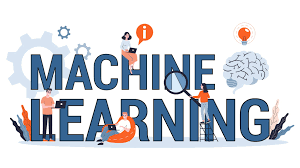
\includegraphics[width=600pt,height=350pt]{img/00-presentacion/machine-learning2} \end{center}

\hypertarget{instructores}{%
\section*{Instructores}\label{instructores}}
\addcontentsline{toc}{section}{Instructores}

\textbf{ACT. ARTURO BRINGAS}

\textbf{LinkedIn:} \href{https://www.linkedin.com/in/arturo-bringas/}{arturo-bringas}
\textbf{Email:} \href{mailto:act.arturo.b@ciencias.unam.mx}{\nolinkurl{act.arturo.b@ciencias.unam.mx}}

Actuario egresado de la Facultad de Ciencias con maestría en Ciencia de Datos por el ITAM.
Se especializa en modelos predictivos y de clasificación de \emph{machine learning} aplicado a seguros, banca, marketing, deportes, e-commerce y movilidad internacional. Ha sido consultor \emph{Senior Data Scientist} para empresas y organizaciones como GNP, El Universal, UNAM, la Organización de las Naciones Unidas Contra la Droga y el Delito (UNODC), entre otros. Actualmente es profesor de \emph{Ciencia de datos y Machine Learning} en AMAT y \emph{Data Scientist Expert} en BBVA, en donde implementa soluciones de analítica avanzada con impacto global.

\begin{center}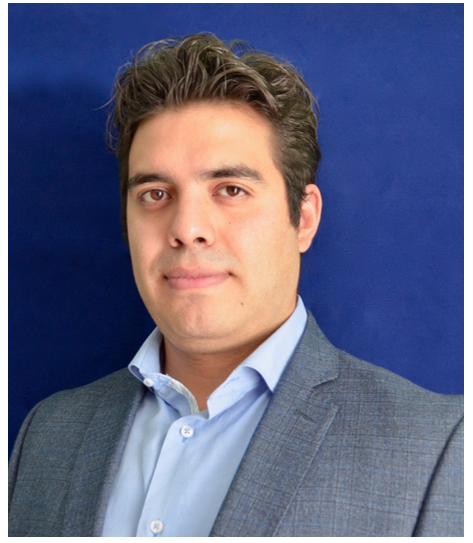
\includegraphics[width=250pt]{img/00-presentacion/arturo} \end{center}

\textbf{ACT. KARINA LIZETTE GAMBOA}

\textbf{LinkedIn:} \href{https://www.linkedin.com/in/kalizzygam/}{KaLizzyGam}
\textbf{Email:} \href{mailto:lizzygamboa@ciencias.unam.mx}{\nolinkurl{lizzygamboa@ciencias.unam.mx}}

Actuaria egresada de la Facultad de Ciencias y candidata a Maestra en
Ciencia de Datos por el ITAM.

Experiencia en áreas de analítica predictiva e inteligencia del negocio. Lead y Senior
Data Scientist en consultoría en diferentes sectores como tecnología, asegurador,
financiero y bancario. Es experta en entendimiento de negocio para la correcta
implementación de algoritmos de inteligencia y explotación de datos.
Actualmente se desarrolla como Arquitecta de Soluciones Analíticas en Merama,
startup mexicana clasificada como uno de los nuevos unicornios de Latinoamérica.
Senior Data Science en CLOSTER y como profesora del diplomado de Metodología
de la Investigación Social por la UNAM así como instructora de cursos de Ciencia de
Datos en AMAT.

Empresas anteriores: GNP, Actinver Banco y Casa de Bolsa, PlayCity Casinos,
RakenDataGroup Consulting, entre otros.

\begin{center}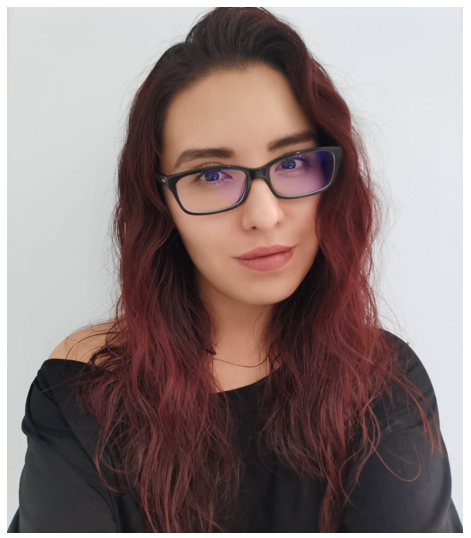
\includegraphics[width=250pt]{img/00-presentacion/lizzy} \end{center}

\hypertarget{alcances-del-curso}{%
\section*{Alcances del curso}\label{alcances-del-curso}}
\addcontentsline{toc}{section}{Alcances del curso}

Al finalizar este curso el participante será capaz de consumir, manipular y visualizar información proveniente de diversas fuentes de información para resolver problemas de propósito general asociados a los datos.

Requisitos:

\begin{itemize}
\tightlist
\item
  Computadora con al menos 8Gb Ram
\item
  Instalar la versión más reciente de R
\item
  Instalar la versión más reciente de RStudio
\end{itemize}

\hypertarget{temario}{%
\subsection*{Temario:}\label{temario}}
\addcontentsline{toc}{subsection}{Temario:}

\textbf{1. Introducción a Ciencia de Datos}

\begin{itemize}
\tightlist
\item
  Machine Learning, Bigdata, BI, AI y CD
\item
  Objetivo de ciencia de datos
\item
  Requisitos y aplicaciones
\item
  Tipos de algoritmos
\item
  Ciclo de vida de un proyecto
\end{itemize}

\textbf{2. Manipulación de datos con Tidyverse}

\begin{itemize}
\tightlist
\item
  Importación de tablas (readr)
\item
  Consultas (dplyr)
\item
  Transformación de estructuras (tidyr)
\end{itemize}

\textbf{3. Concepto de Machine Learning}

\begin{itemize}
\tightlist
\item
  Machine learning
\item
  Análisis supervisado
\item
  Análisis no supervisado
\item
  Sesgo y varianza
\item
  Partición de datos
\item
  Preprocesamiento e ingeniería de datos
\end{itemize}

\textbf{4. Algoritmos de Machine Learning}

\begin{itemize}
\tightlist
\item
  Clustering: Kmeans, kmedoids, agnes
\item
  Regresión Lineal
\item
  Métricas de error
\item
  Regresión logística
\item
  Métricas de error
\item
  KNN
\item
  Árbol de decisión
\item
  Random Forest
\item
  Comparación de modelos
\end{itemize}

\hypertarget{duraciuxf3n-y-evaluaciuxf3n-del-curso}{%
\section*{Duración y evaluación del curso}\label{duraciuxf3n-y-evaluaciuxf3n-del-curso}}
\addcontentsline{toc}{section}{Duración y evaluación del curso}

\begin{itemize}
\item
  El programa tiene una duración de 40 hrs.
\item
  Las clases serán impartidas los días sábado, de 9:00 am a 1:00 pm
\item
  Serán asignados ejercicios que el participante deberá resolver entre una semana y otra.
\item
  Al final del curso se solicitará un proyecto final, el cual deberá ser entregado para ser acreedor a la constancia de participación.
\end{itemize}

\hypertarget{recursos-y-dinuxe1mica-de-clase}{%
\section*{Recursos y dinámica de clase}\label{recursos-y-dinuxe1mica-de-clase}}
\addcontentsline{toc}{section}{Recursos y dinámica de clase}

En esta clase estaremos usando:

\begin{itemize}
\tightlist
\item
  R \href{https://cran.r-project.org/}{da click aquí si aún no lo descargas}
\item
  RStudio \href{https://www.rstudio.com/products/rstudio/download/}{da click aquí también}
\item
  Miro \href{https://miro.com/welcomeonboard/WXJiSGtOUnE4Mm1EQnJaQWxIR2R6RGxPaVo5eXQ3bG1SMHNWSkVIZ09YQ3JlTHRma1dYcFJzbm9wZ05OVmxVMXwzMDc0NDU3MzU1MzI0OTQwMDI5?invite_link_id=632956861297}{úsame}
\item
  Zoom \href{https://us02web.zoom.us/j/5155440751?pwd=YzJCOGF0VnlZdlZlS0Fpc3MvZEhadz09}{Clases}

  \begin{itemize}
  \tightlist
  \item
    Pulgar arriba: Voy bien, estoy entendiendo!
  \item
    Pulgar abajo: Eso no quedó muy claro
  \item
    Mano arriba: Quiero participar/preguntar ó Ya estoy listo para iniciar
  \end{itemize}
\item
  Grupo de WhatsApp \href{https://chat.whatsapp.com/CNv5RxZb7FnLbzUFHGtYMG}{El chismecito está aquí}
\item
  \href{https://drive.google.com/drive/u/1/folders/16aKNbkhYfF-x6R2oh4RswSQOXN62UQX3}{One Drive}
\item
  Notas de clase \href{KaLizzyGam.github.io/index.html}{Revisame si quieres aprender}
\end{itemize}

\hypertarget{conceptos-de-ciencia-de-datos}{%
\chapter{Conceptos de Ciencia de Datos}\label{conceptos-de-ciencia-de-datos}}

\hypertarget{quuxe9-es-ciencia-de-datos}{%
\section{¿Qué es Ciencia de Datos?}\label{quuxe9-es-ciencia-de-datos}}

\begin{center}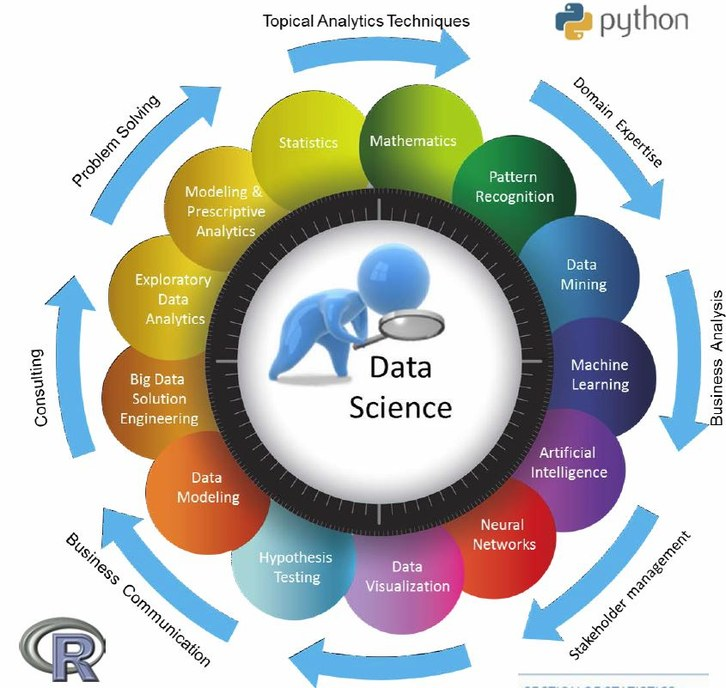
\includegraphics[width=500pt,height=500pt]{img/01-intro2ds/01_data-science-applications} \end{center}

\hypertarget{definiendo-conceptos}{%
\subsection*{Definiendo conceptos:}\label{definiendo-conceptos}}
\addcontentsline{toc}{subsection}{Definiendo conceptos:}

\textbf{Estadística} Disciplina que recolecta, organiza, analiza e interpreta datos. Lo hace a través de una población muestral generando estadística descriptiva y estadística inferencial.

\begin{itemize}
\item
  La \href{}{estadística descriptiva}, como su nombre lo indica, se encarga de describir datos y obtener conclusiones. Se utilizan números (media, mediana, moda, mínimo, máximo, etc) para analizar datos y llegar a conclusiones de acuerdo a ellos.
\item
  La \href{}{estadística inferencial} argumenta o infiere sus resultados a partir de las muestras de una población. Se intenta conseguir información al utilizar un procedimiento ordenado en el manejo de los datos de la muestra.
\item
  La \href{}{estadística predictiva} busca estimar valores y escenarios futuros más probables de ocurrir a partir de referencias históricas previas. Se suelen ocupar como apoyo características y factores áltamente asociados al fenómeno que se desea predecir.
\end{itemize}

\begin{center}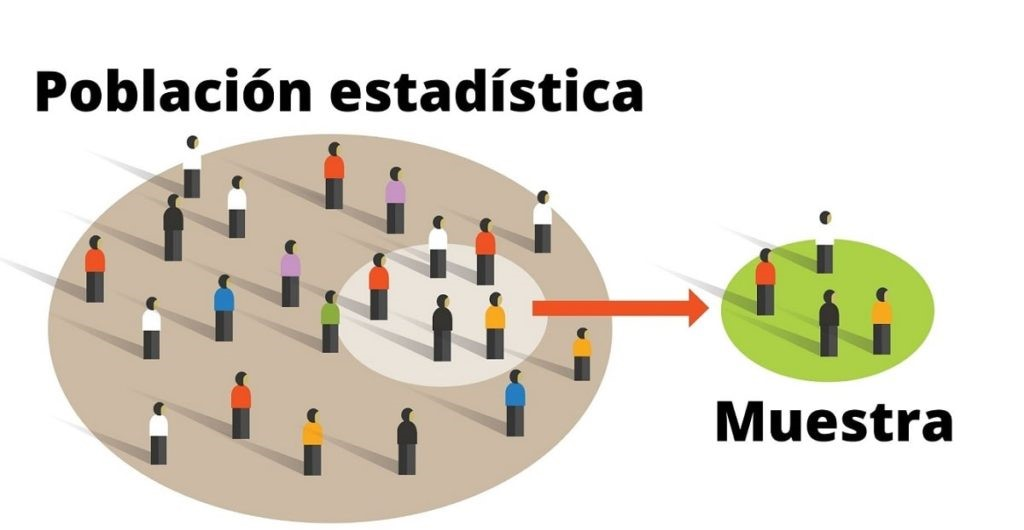
\includegraphics{img/01-intro2ds/02_muestra} \end{center}

\textbf{Business Intelligence}: BI aprovecha el software y los servicios para transformar los datos en conocimientos prácticos que informan las decisiones empresariales estratégicas y tácticas de una organización. Las herramientas de BI acceden y analizan conjuntos de datos y presentan hallazgos analíticos en informes, resúmenes, tableros, gráficos, cuadros, -indicadores- o KPI's y mapas para proporcionar a los usuarios \textbf{inteligencia detallada sobre el estado del negocio}. BI esta enfocado en analizar la historia pasada para tomar decisiones hacia el futuro.

¿Qué características tiene un KPI?

\begin{itemize}
\tightlist
\item
  Específicos
\item
  Continuos y periódicos
\item
  Objetivos
\item
  Cuantificables
\item
  Medibles
\item
  Realistas
\item
  Concisos
\item
  Coherentes
\item
  Relevantes
\end{itemize}

\begin{center}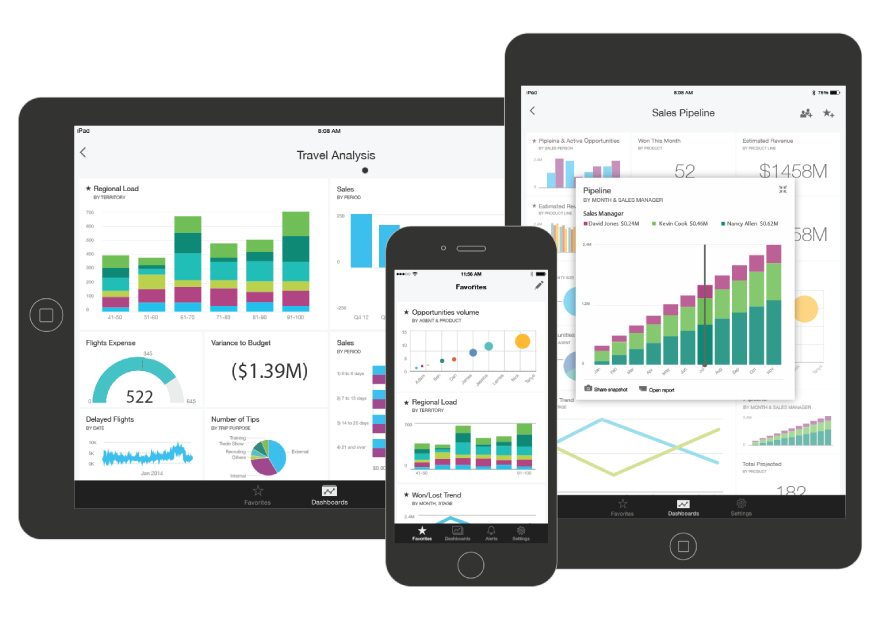
\includegraphics{img/01-intro2ds/03_bi} \end{center}

\textbf{Machine Learning}: Machine learning --aprendizaje de máquina-- es una \textbf{rama de la inteligencia artificial} que permite que las máquinas aprendan de los patrones existentes en los datos. Se usan métodos computacionales para aprender de datos con el fin de producir reglas para mejorar el desempeño en alguna tarea o toma de decisión. (Está enfocado en la programación de máquinas para aprender de los patrones existentes en datos principalmente estructurados y anticiparse al futuro)

\begin{center}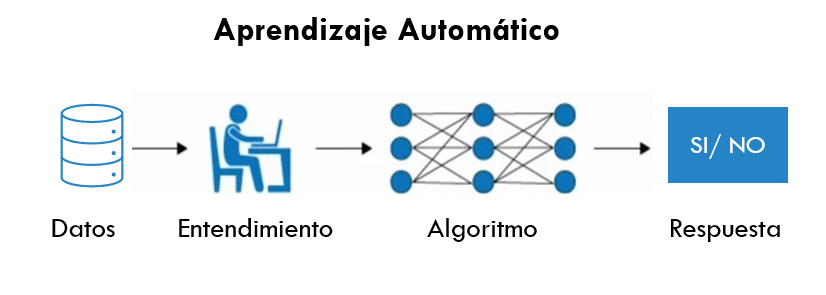
\includegraphics[width=600pt]{img/01-intro2ds/04_ml} \end{center}

\begin{center}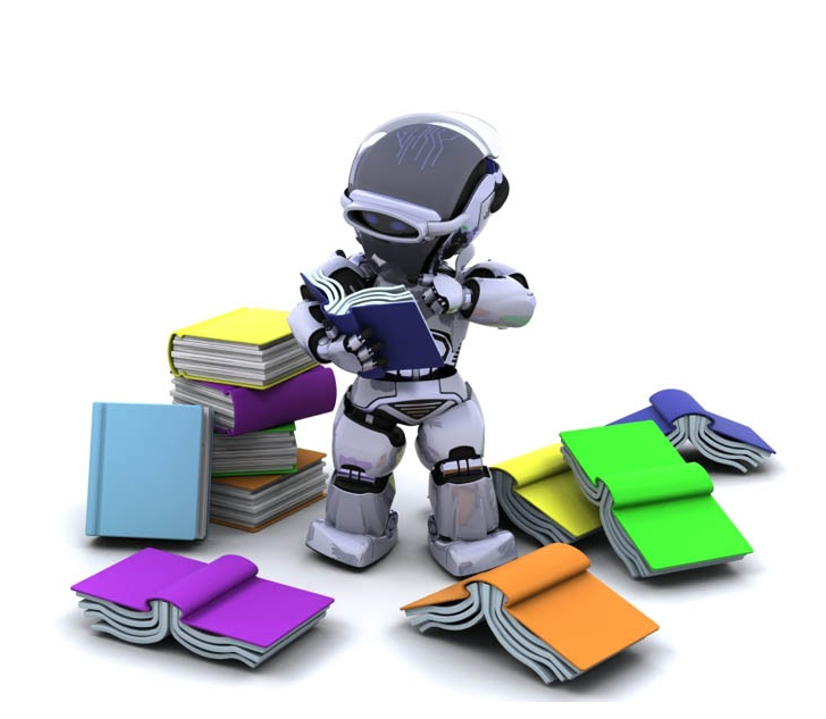
\includegraphics{img/01-intro2ds/05_supervisado_robo} \end{center}

\textbf{Deep Learning}: El aprendizaje profundo es un subcampo del aprendizaje automático que se ocupa de los algoritmos \textbf{inspirados en la estructura y función del cerebro llamados redes neuronales artificiales.}

En \emph{Deep Learning}, un modelo de computadora aprende a realizar tareas de clasificación directamente a partir de imágenes, texto o sonido. Los modelos de aprendizaje profundo pueden lograr una precisión de vanguardia, a veces superando el rendimiento a nivel humano. Los modelos se entrenan mediante el uso de un gran conjunto de datos etiquetados y arquitecturas de redes neuronales que contienen muchas capas. (Está enfocado en la programación de máquinas para el reconocimiento de imágenes y audio (datos no estructurados))

\begin{center}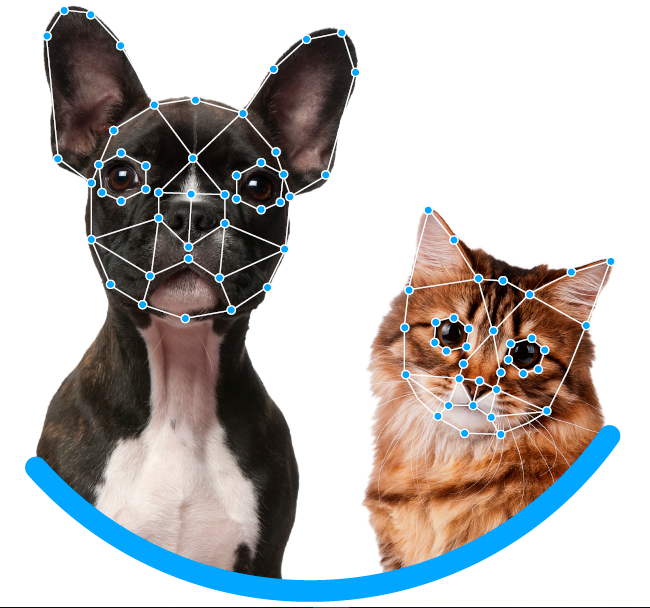
\includegraphics{img/01-intro2ds/06_reconocimiento} \end{center}

\begin{center}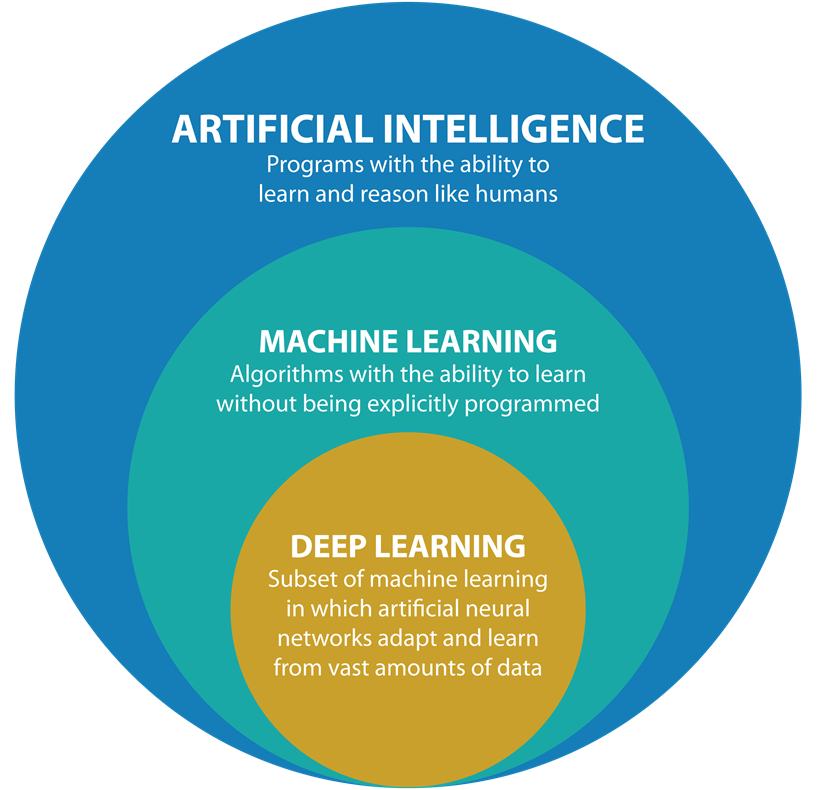
\includegraphics{img/01-intro2ds/07_ml1} \end{center}

\textbf{Big data} se refiere a los grandes y diversos conjuntos de información que crecen a un ritmo cada vez mayor. Abarca el volumen de información, la velocidad a la que se crea y recopila, y la variedad o alcance de los puntos de datos que se cubren. Los macrodatos a menudo provienen de la minería de datos y llegan en múltiples formatos.

\begin{center}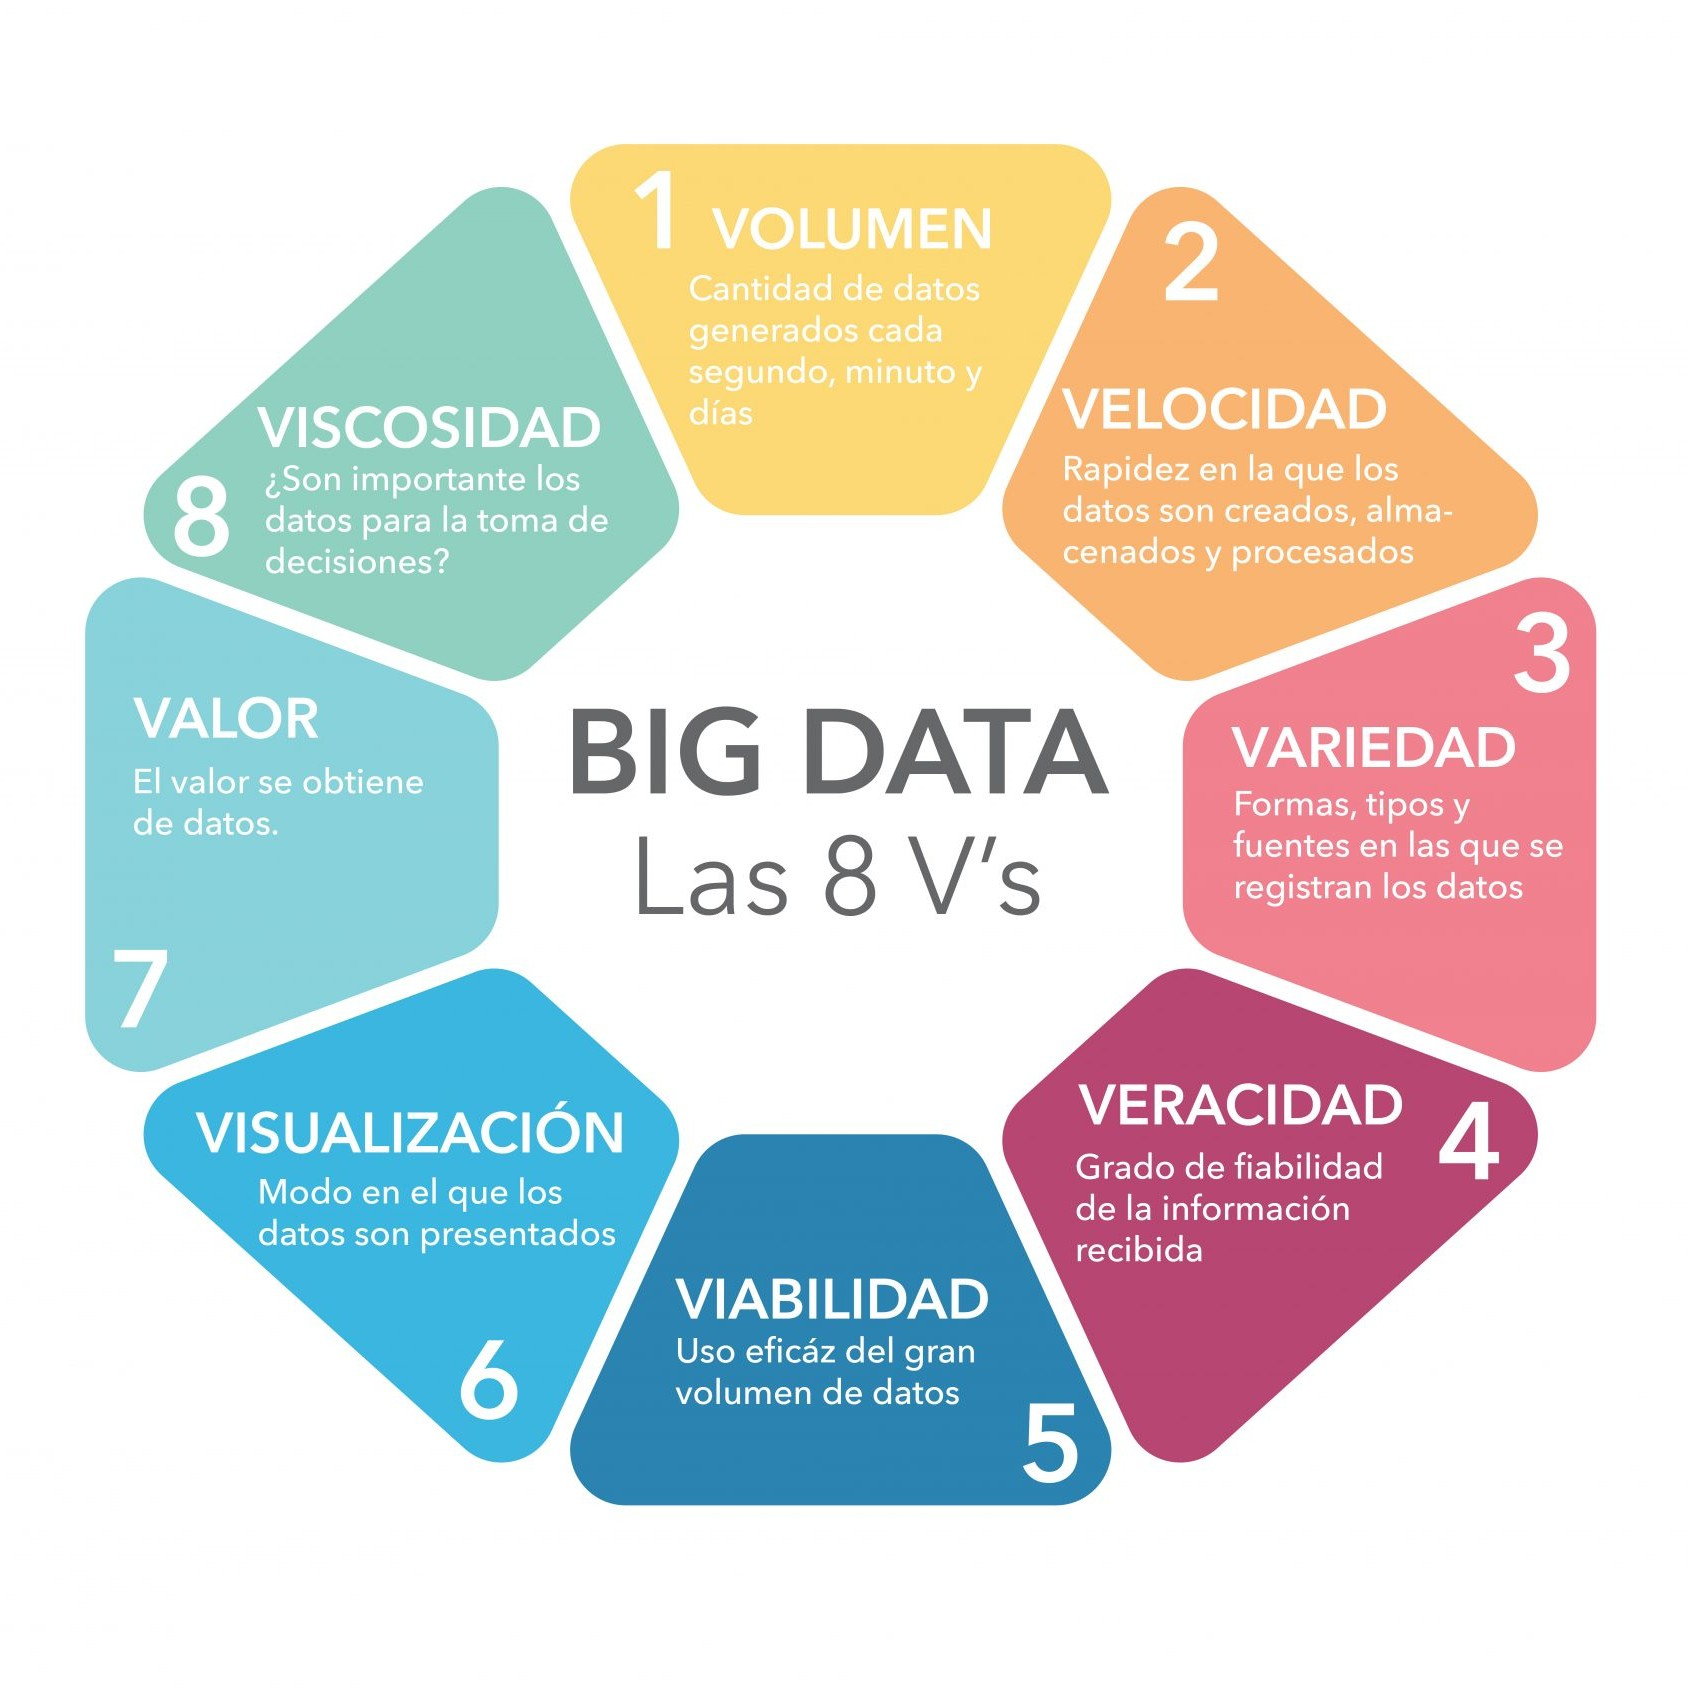
\includegraphics[width=600pt]{img/01-intro2ds/08_big-data-8vs} \end{center}

Es común que se confunda los conceptos de \emph{Big Data} y \emph{Big Compute}, como se mencionó, \emph{Big Data} se refiere al procesamiento de conjuntos de datos que son más voluminosos y complejos que los tradicionales y \emph{Big Compute} a herramientas y enfoques que utilizan una gran cantidad de recursos de CPU y memoria de forma coordinada para resolver problemas que usan algoritmos muy complejos.

\begin{center}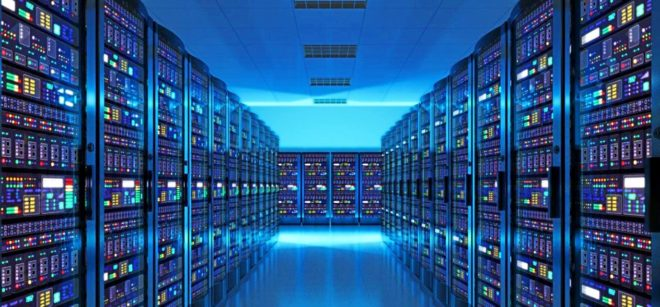
\includegraphics[width=600pt]{img/01-intro2ds/09_bigdata} \end{center}

Curiosidad: \href{https://www.xatakawindows.com/actualidad-en-redmond/servidores-liquido-hirviendo-esta-idea-microsoft-para-evitar-calentamiento-sus-equipos\#:~:text=Con\%20este\%20sistema\%2C\%20el\%20dispositivo,fr\%C3\%ADo\%2C\%20emplea\%20uno\%20en\%20ebullici\%C3\%B3n.}{Servidores en líquido para ser enfriados}

Curiosidad 2: \href{https://www.bbc.com/mundo/noticias/2016/02/160202_microsoft_centro_datos_debajo_agua_mar_subamino_all}{Centro de datos en el océano}

\textbf{Entonces, ¿qué NO es ciencia de datos?}

\begin{itemize}
\tightlist
\item
  No es una tecnología
\item
  No es una herramienta
\item
  No es desarrollo de software
\item
  No es Business Intelligence*
\item
  No es Big Data*
\item
  No es Inteligencia Artificial*
\item
  No es (solo) machine learning
\item
  No es (solo) deep learning
\item
  No es (solo) visualización
\item
  No es (solo) hacer modelos
\end{itemize}

\hypertarget{objetivos}{%
\section{Objetivos}\label{objetivos}}

\begin{itemize}
\tightlist
\item
  Los científicos de datos analizan qué preguntas necesitan respuesta y dónde encontrar los datos relacionados. Tienen conocimiento de negocio y habilidades analíticas, así como la capacidad de extraer, limpiar y presentar datos. Las empresas utilizan científicos de datos para obtener, administrar y analizar grandes cantidades de datos no estructurados. Luego, los resultados se sintetizan y comunican a las partes interesadas clave para impulsar la toma de decisiones estratégicas en la organización.
\end{itemize}

\begin{center}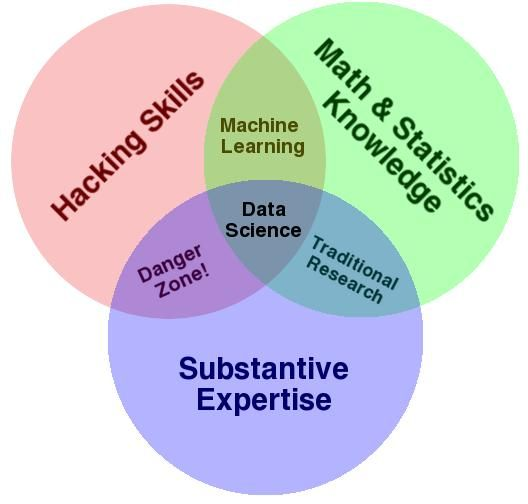
\includegraphics[width=600pt,height=500pt]{img/01-intro2ds/10_data_science_vd} \end{center}

Fuente: \href{http://drewconway.com/zia/2013/3/26/the-data-science-venn-diagram}{Blog post de Drew Conway}

Más sobre Conway: \href{https://www.forbes.com/sites/joshwolfe/2016/03/03/using-data-science-for-the-physical-world/?sh=614ac5b0150e}{Forbes 2016}

\hypertarget{requisitos}{%
\section{Requisitos}\label{requisitos}}

\begin{itemize}
\item
  \textbf{Background científico:} Conocimientos generales de probabilidad, estadística, álgebra lineal, cálculo, geometría analítica, programación, conocimientos computacionales\ldots{} etc
\item
  \textbf{Datos relevantes y suficientes:} Es indispensable saber si los datos con los que se trabajará son relevantes y suficientes, debemos evaluar qué preguntas podemos responder con los datos con los que contamos.

  \begin{itemize}
  \item
    \textbf{Suficiencia:} Los datos con los que trabajamos tienen que ser representativos de la población en general, necesitamos que las características representadas en la información sean suficientes para aproximar a la población objetivo.
  \item
    \textbf{Relevancia:} De igual manera los datos tienen que tener relevancia para la tarea que queremos resolver, por ejemplo, es probable que información sobre gusto en alimentos sea irrelevante para predecir número de hijos.
  \end{itemize}
\end{itemize}

\begin{center}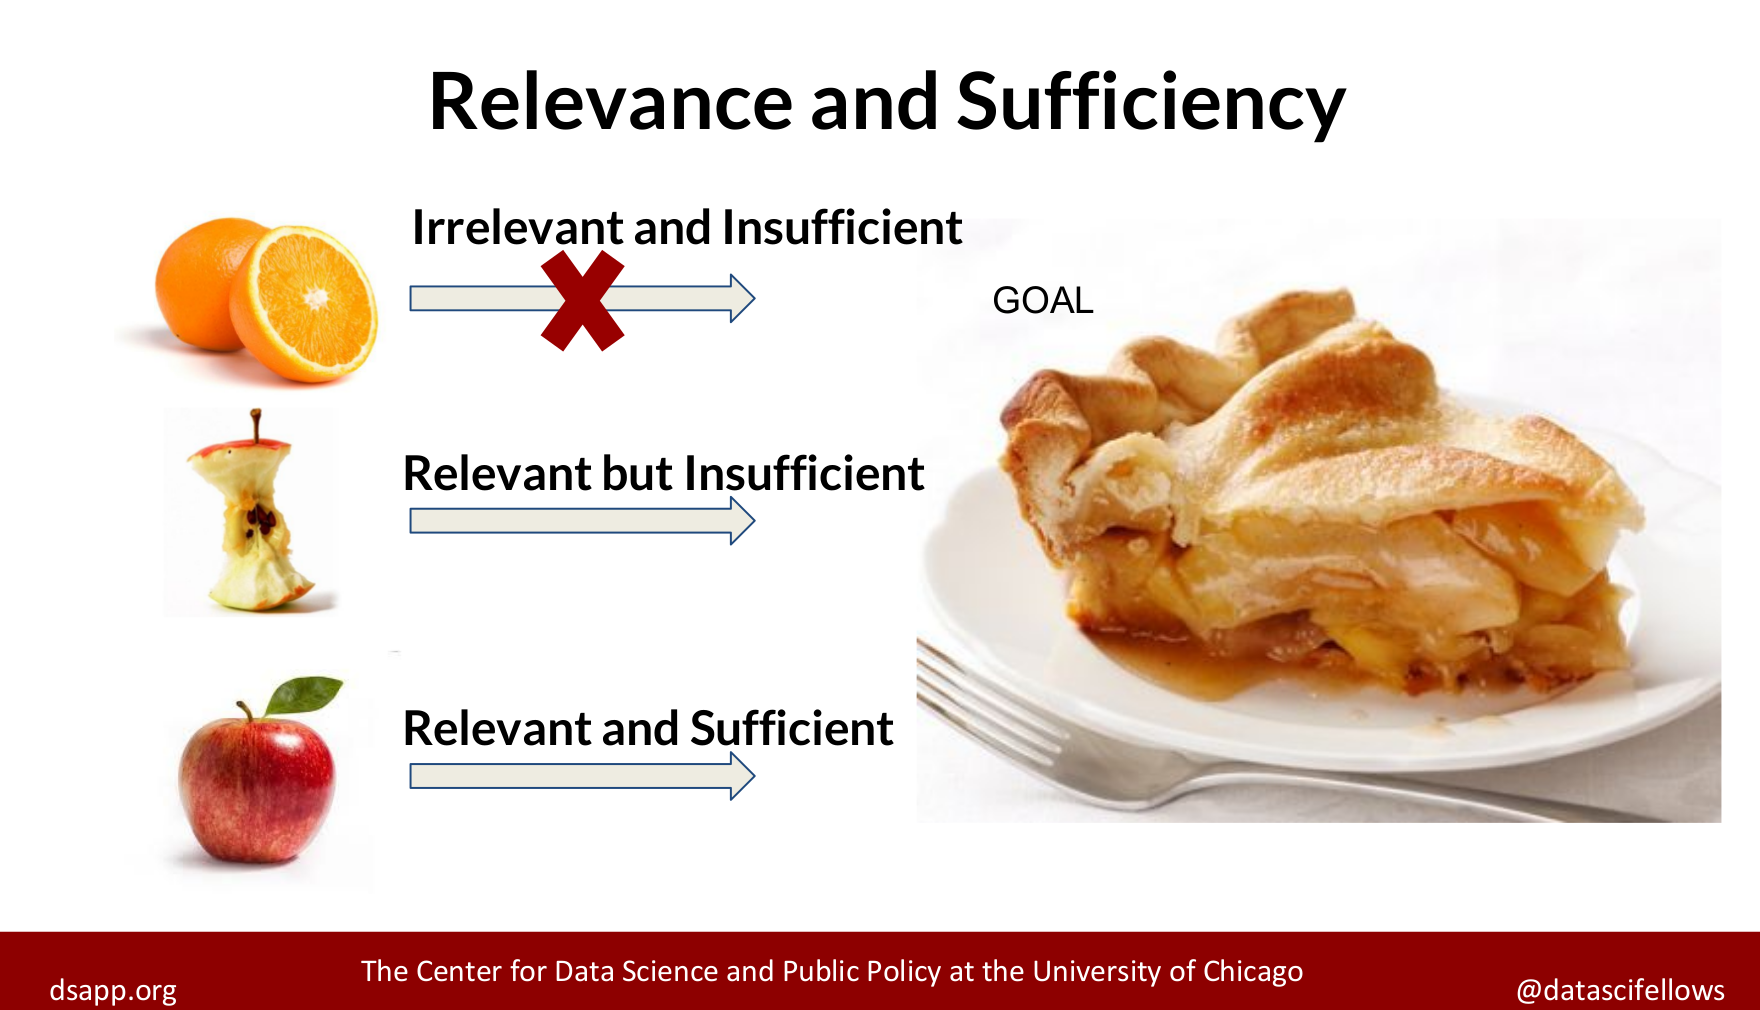
\includegraphics{img/01-intro2ds/11_relevancia_suficiencia} \end{center}

\begin{itemize}
\tightlist
\item
  \textbf{Etiquetas:} Se necesita la intervención humana para etiquetar, clasificar e introducir los datos en el algoritmo.
\end{itemize}

\begin{center}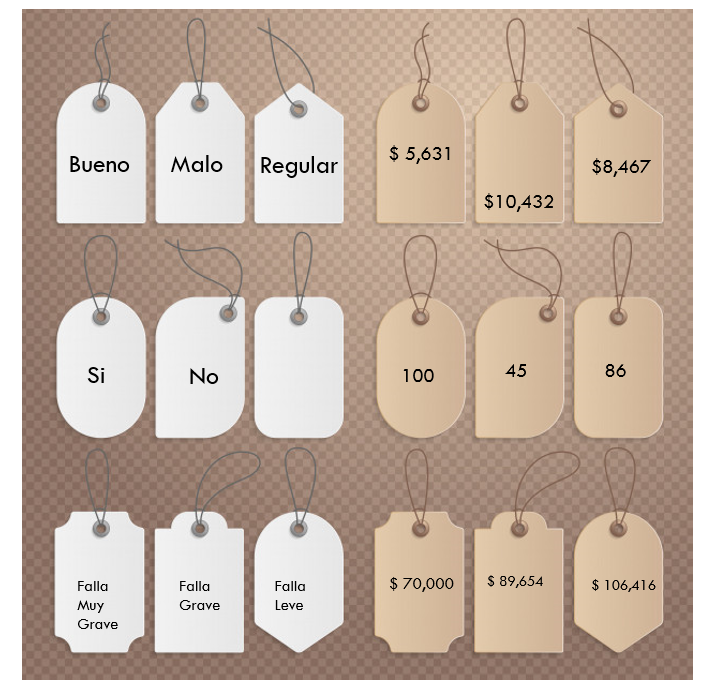
\includegraphics[width=600pt,height=400pt]{img/01-intro2ds/12_etiquetas} \end{center}

\begin{itemize}
\tightlist
\item
  \textbf{Software:} Existen distintos lenguajes de programación para realizar ciencia de datos
\end{itemize}

\begin{center}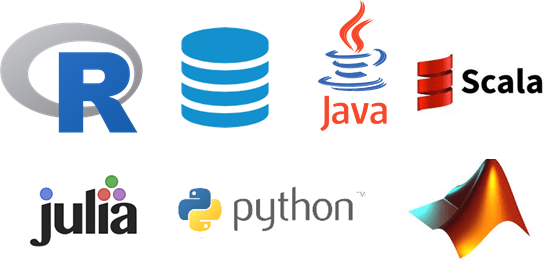
\includegraphics[width=600pt,height=300pt]{img/01-intro2ds/13_lenguajes} \end{center}

\hypertarget{aplicaciones}{%
\section{Aplicaciones}\label{aplicaciones}}

Dependiendo de la industria en la que se quiera aplicar Machine Learning, podemos pensar en distintos enfoques, en la siguiente imagen se muestran algunos ejemplos:

\begin{center}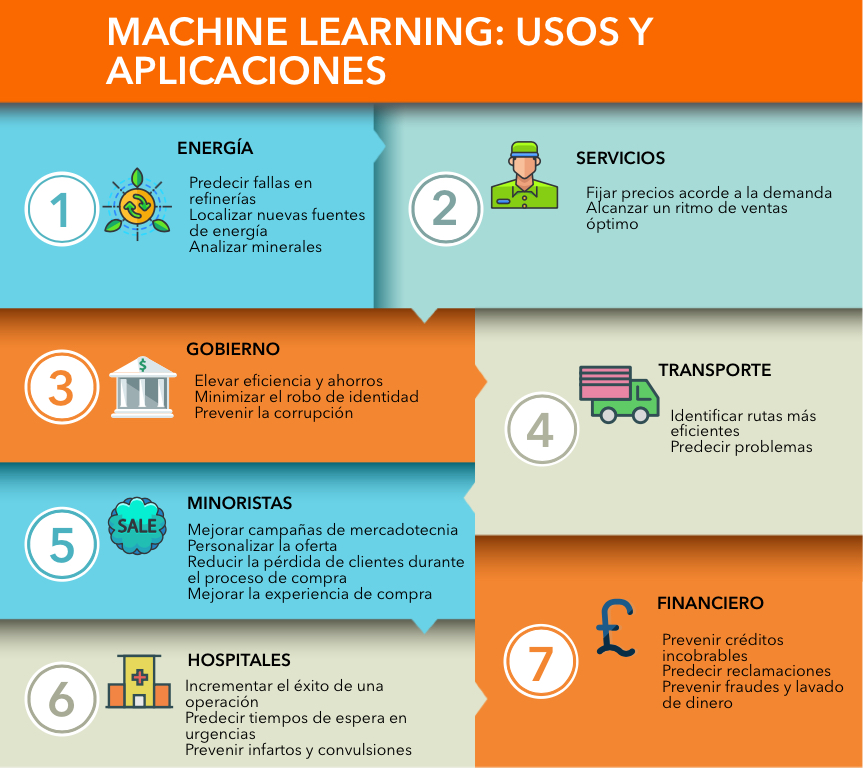
\includegraphics[width=600pt,height=600pt]{img/01-intro2ds/14_aplicaciones} \end{center}

Podemos pensar en una infinidad de aplicaciones comerciales basadas en el análisis de datos. Con la intención de estructurar las posibles aplicaciones, se ofrece a continuación una categorización que, aunque no es suficiente para englobar todos los posibles casos de uso, sí es sorprendente la cantidad de aplicaciones que abarca.

\textbf{1. Aplicaciones centradas en los clientes}

\begin{itemize}
\tightlist
\item
  Incrementar beneficio al mejorar recomendaciones de productos
\item
  Up-selling
\item
  Cross-selling
\item
  Reducir tasas de cancelación y mejorar tasas de retención
\item
  Personalizar experiencia de usuario
\item
  Mejorar el marketing dirigido
\item
  Análisis de sentimientos
\item
  Personalización de productos o servicios
\end{itemize}

\textbf{2. Optimización de problemas}

\begin{itemize}
\tightlist
\item
  Optimización de precios
\item
  Ubicación de nuevas sucursales
\item
  Maximización de ganancias mediante producción de materias primas
\item
  Construcción de portafolios de inversión
\end{itemize}

\textbf{3. Predicción de demanda}

\begin{itemize}
\tightlist
\item
  Número futuro de clientes
\item
  Número esperado de viajes en avión / camión / bicis
\item
  Número de contagios por un virus (demanda médica / medicamentos / etc)
\item
  Predicción de uso de recursos (luz / agua / gas)
\end{itemize}

\textbf{4. Análisis de detección de fraudes}

\begin{itemize}
\tightlist
\item
  Detección de robo de identidad
\item
  Detección de transacciones ilícitas
\item
  Detección de servicios fraudulentos
\item
  Detección de zonas geográficas con actividades ilícitas
\end{itemize}

  \bibliography{book.bib,packages.bib}

\end{document}
